\documentclass[12pt,a4paper,UTF8]{article}
\usepackage{circuit} % 格式控制
\graphicspath{{./figures/}} % 指定图片所在文件夹  
% 正文开始
\begin{document}
    % 单图
    \begin{figure}[!htbp]
        \centering
        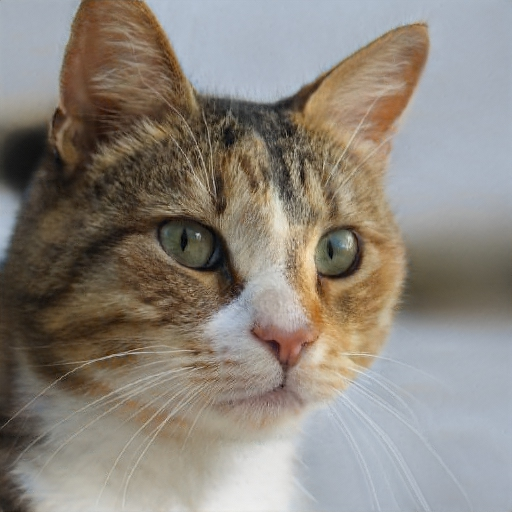
\includegraphics[width=0.8\textwidth]{example}
        \caption{单图排版}
    \end{figure}

    % fig.tex
    % 双图并排非子图
    \begin{figure}[!htbp]
        \centering
        \begin{minipage}[b]{0.45\linewidth}
            \centering
            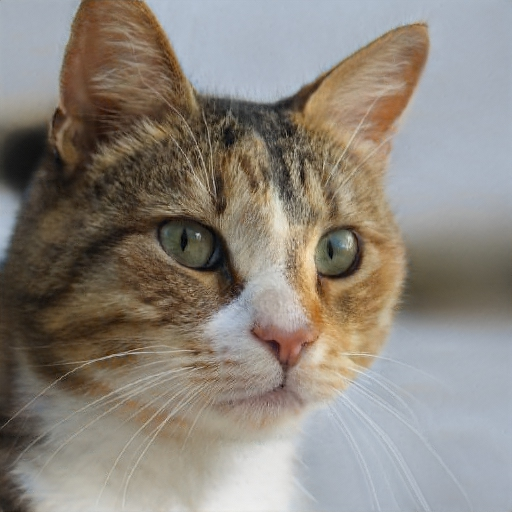
\includegraphics[width=0.9\textwidth]{example}
            \caption{非子图并排题注1}
             
        \end{minipage}%
        \begin{minipage}[b]{0.45\linewidth}
            \centering
            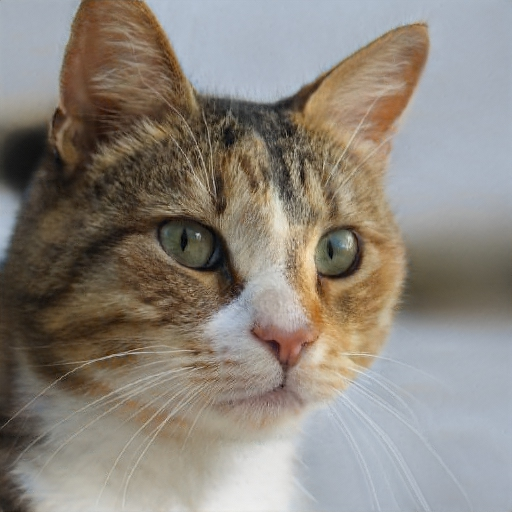
\includegraphics[width=0.9\textwidth]{example}
            \caption{非子图并排题注2}
             
        \end{minipage}
    \end{figure}

    % fig.tex
    % 双图并排子图
    \begin{figure}[!htbp]
        \centering
        \subcaptionbox{双图并排子图1}[0.45\textwidth][c]{
            \centering
            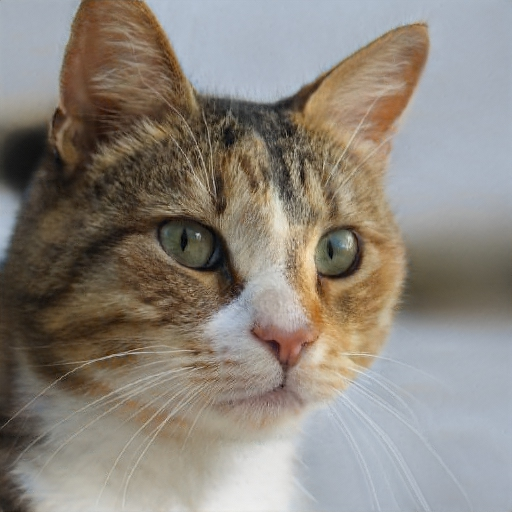
\includegraphics[width=0.4\textwidth]{example}
             
        }%
        \hspace{0.5cm} 
        \subcaptionbox{双图并排子图1}[0.45\textwidth][c]{
            \centering
            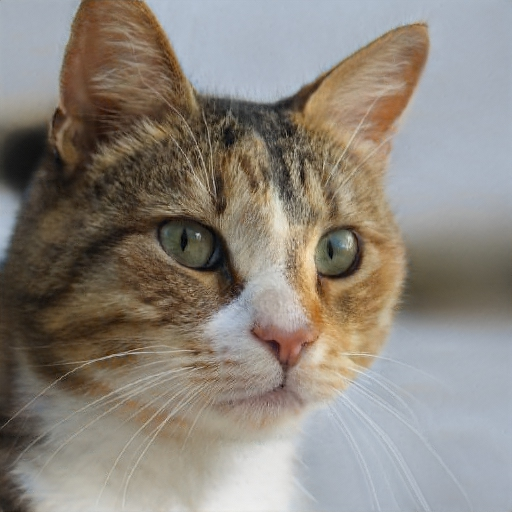
\includegraphics[width=0.4\textwidth]{example}
             
        } 
        \caption{双图并排子图}
         
    \end{figure}


    % 双图纵排子图
    % fig.tex
    \begin{figure}[!htbp]
        \centering
        \subcaptionbox{双图纵排子图1}[0.45\textwidth][c]{
            \centering
            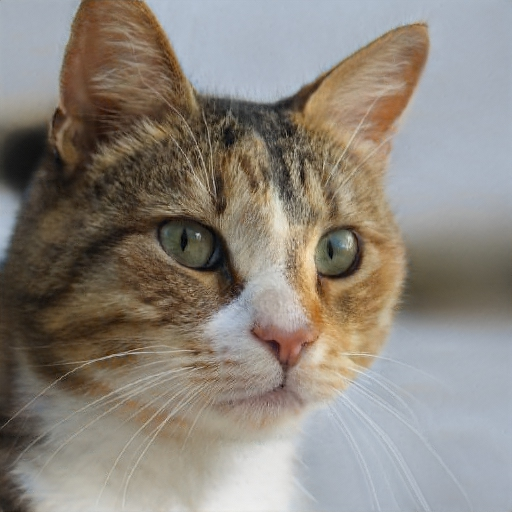
\includegraphics[width=0.4\textwidth]{example}
             
        }\\[0.5cm]% % 换行并产生图片纵向距离
        \subcaptionbox{双图纵排子图2}[0.45\textwidth][c]{
            \centering
            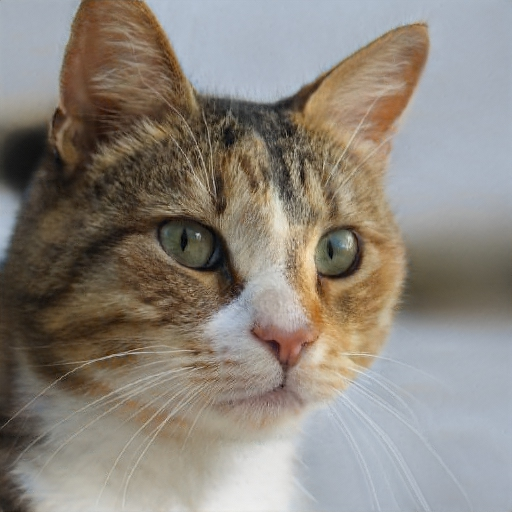
\includegraphics[width=0.4\textwidth]{example}
             
        } 
        \caption{双图纵排子图}
         
    \end{figure}
    
    % 三个子图横排
    % fig.tex
    \begin{figure}[!htbp]
        \centering
        \subcaptionbox{三个子图横排1}[0.33\textwidth][c]{
            \centering
            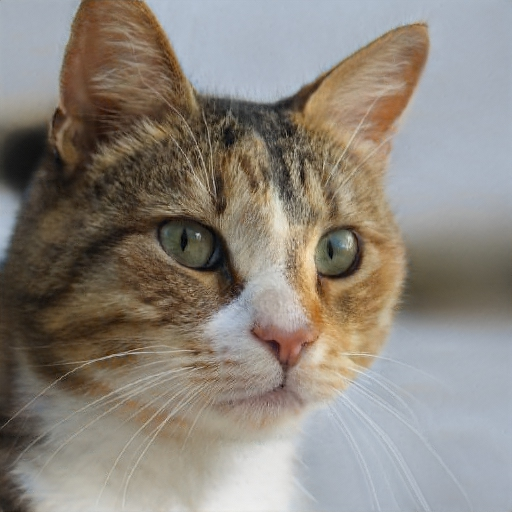
\includegraphics[width=0.32\textwidth]{example}
             
        }%
            \subcaptionbox{三个子图横排2}[0.33\textwidth][c]{
            \centering
            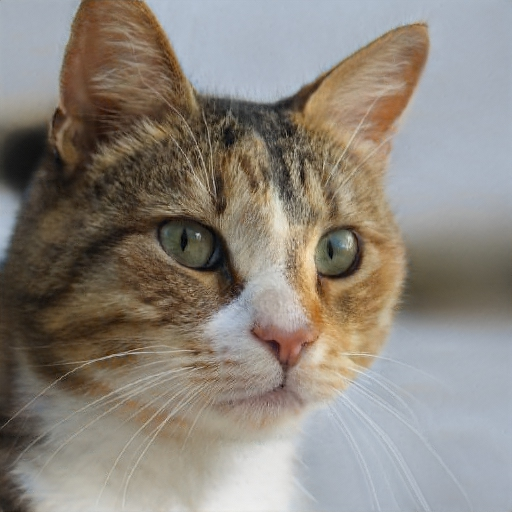
\includegraphics[width=0.32\textwidth]{example}
             
        }%
            \subcaptionbox{三个子图横排3}[0.33\textwidth][c]{
            \centering
            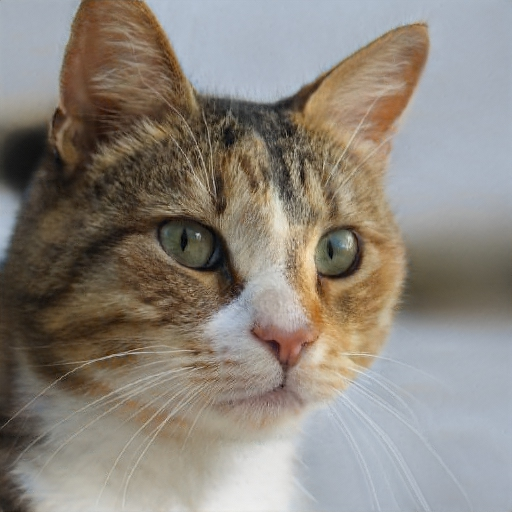
\includegraphics[width=0.32\textwidth]{example}
             
        }%
        \caption{三个子图横排}
         
    \end{figure}

    % 三个子图1+2模式
    % fig.tex
    \begin{figure}[!htbp]
        \centering
        \subcaptionbox{三个子图1+2模式1}[0.45\textwidth][c]{
            \centering
            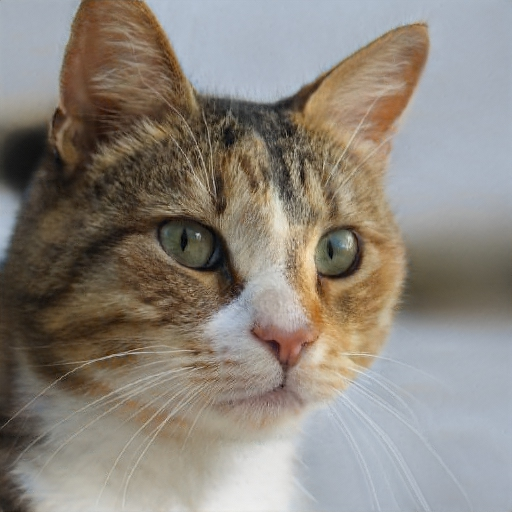
\includegraphics[width=0.45\textwidth]{example}
             
        }\\%
        \subcaptionbox{三个子图1+2模式2}[0.45\textwidth][c]{
            \centering
            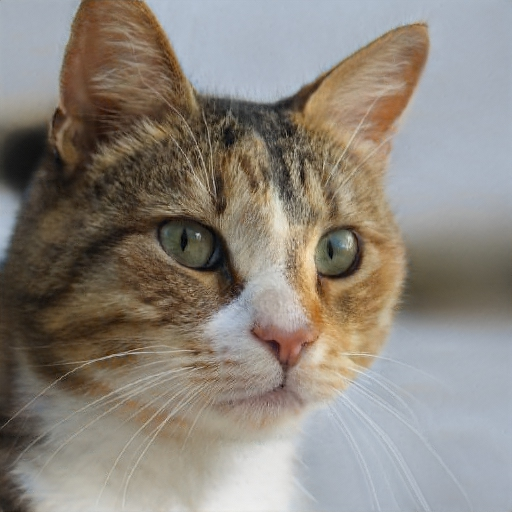
\includegraphics[width=0.45\textwidth]{example}
             
        }%
        \hspace{0.3cm}
        \subcaptionbox{三个子图1+2模式3}[0.45\textwidth][c]{
            \centering
            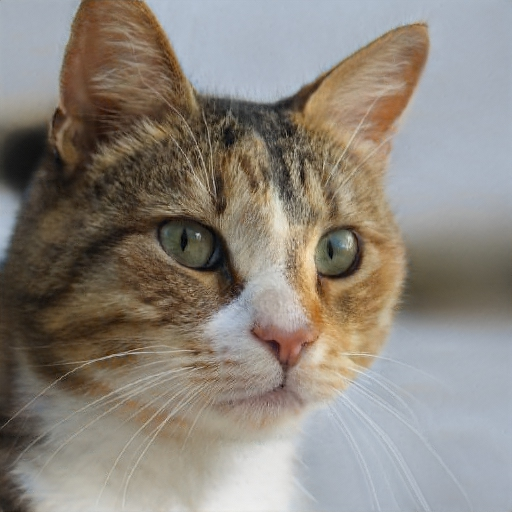
\includegraphics[width=0.45\textwidth]{example}
             
        }%
        \caption{三个子图1+2模式}
         
    \end{figure}



    % 三个子图一大两小
    % fig.tex
    \begin{figure}[!htbp]
        \centering
        \begin{minipage}[b]{0.45\textwidth}
            \centering
            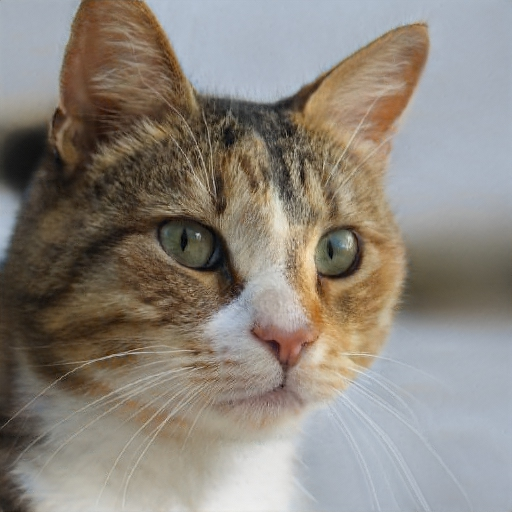
\includegraphics[width=\textwidth, height=1.2\textwidth]{example}
            \caption{三个图非子图一大两小1}
             
        \end{minipage}
        \hspace{0.5cm}%
        \begin{minipage}[b]{0.4\textwidth}
            \begin{minipage}[b]{\textwidth}
                \centering
                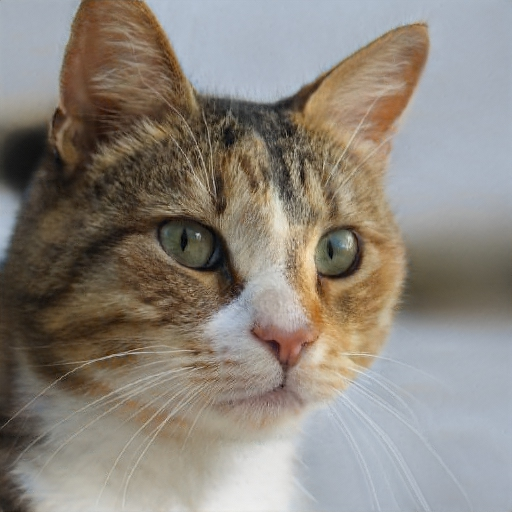
\includegraphics[width=\textwidth]{example}
                \caption{三个图非子图一大两小2}
                 
            \end{minipage}\\[0.8cm]%
            \begin{minipage}[b]{\textwidth}
                \centering
                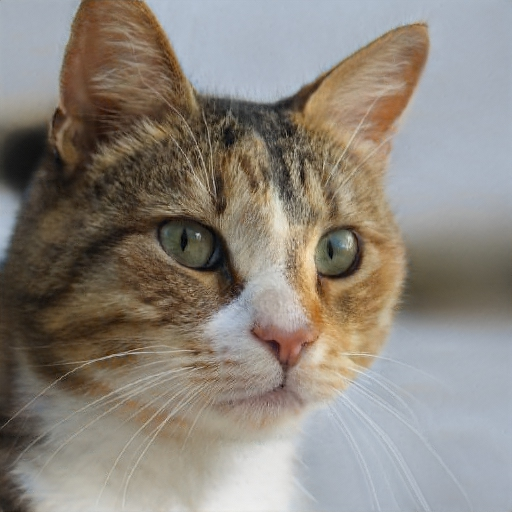
\includegraphics[width=\textwidth]{example}
                \caption{三个图非子图一大两小3}		
                 
            \end{minipage}	
        \end{minipage}
    \end{figure}

    % 四个子图
    % fig.tex
    \begin{figure}[!htbp]
        \centering
        \subcaptionbox{四个子图1}[0.45\textwidth][c]{
            \centering
            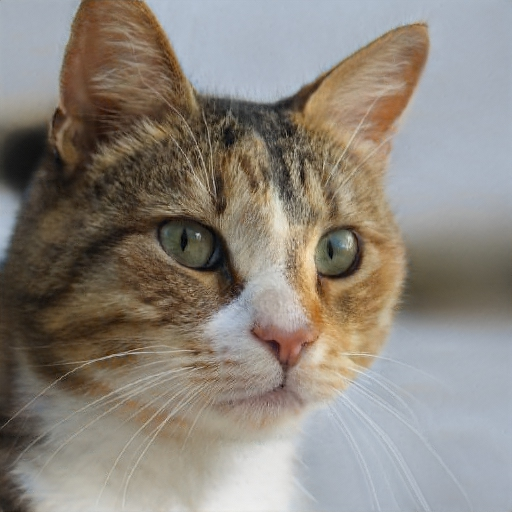
\includegraphics[width=0.45\textwidth]{example}
             
        }%
        \hspace*{0.1cm}
        \subcaptionbox{四个子图2}[0.45\textwidth][c]{
            \centering
            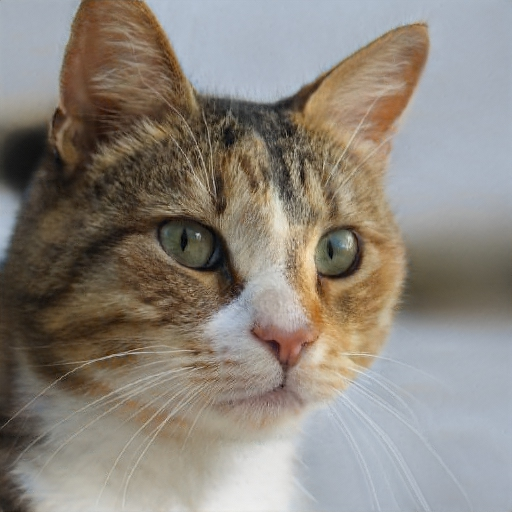
\includegraphics[width=0.45\textwidth]{example}
             
        }\\% % 换行
        \subcaptionbox{四个子图3}[0.45\textwidth][c]{
            \centering
            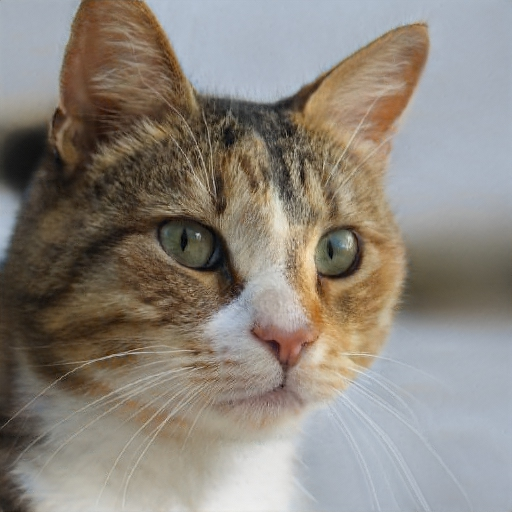
\includegraphics[width=0.45\textwidth]{example}
             
        }%
        \hspace*{0.1cm}
        \subcaptionbox{四个子图4}[0.45\textwidth][c]{
            \centering
            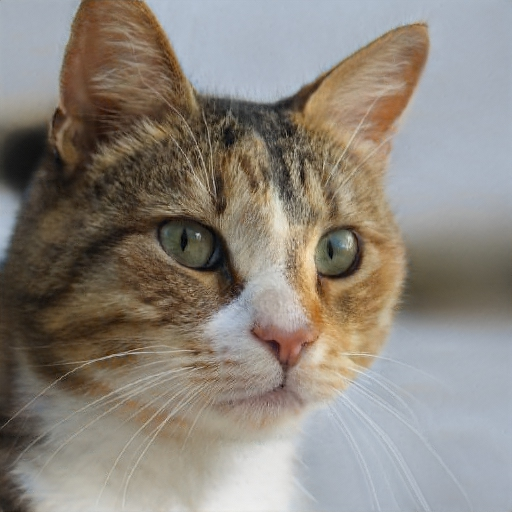
\includegraphics[width=0.45\textwidth]{example}
             
        }%
        \caption{四个子图}
         
    \end{figure}

\end{document}